% !TeX spellcheck = en_US 
%\documentclass[12pt]{amsart}
\documentclass[varwidth]{standalone}
%\documentclass{standalone}
%\usepackage{amsmath, amsthm, amsfonts, amssymb, latexsym}

% required packages
\usepackage{pgfplots, tikz-3dplot, ifthen}


\begin{document}
	

	\begin{figure}
	\begin{center}
	\begin{tikzpicture}[scale=1.0]
		\draw (-2.83,2.83) -- (2.83,-2.83);  % H_1 
		\draw (2.83,2.83) -- (-2.83,-2.83);  % H_2 
		\draw (-1.,3.87) -- (-1.,-3.87);  % H_3 
		\draw (1.,3.87) -- (1.,-3.87);  % H_4 
		\draw (3.87,-1.) -- (-3.87,-1.);  % H_5 
		\draw (3.87,1.) -- (-3.87,1.);  % H_6 
	\end{tikzpicture}
	
	
	\begin{tikzpicture}[scale=1.0]
		\draw[color=red] (-3.56,1.83) -- (1.83,-3.56);  % H_1 
		\node at (1.97,-3.71) {\small $1$}; 
		\draw[color=red] (2.83,2.83) -- (-2.83,-2.83);  % H_2 
		\node at (-2.97,-2.97) {\small $2$}; 
		\draw (3.35,2.16) -- (-4.,0.20);  % H_3 
		\node at (-4.20,0.14) {\small $3$}; 
		\draw (-1.04,3.85) -- (1.04,-3.85);  % H_4 
		\node at (1.09,-4.06) {\small $4$}; 
		\draw (2.16,3.35) -- (0.20,-4.);  % H_5 
		\node at (0.14,-4.20) {\small $5$}; 
		\draw (-3.85,1.04) -- (3.85,-1.04);  % H_6 
		\node at (4.06,-1.09) {\small $6$}; 
		
		\fill[red] (-0.87,-0.87) circle[radius=2pt];  % P[ 1, 2 ] 
		\fill[red] (-2.37,0.63) circle[radius=2pt];  % P[ 1, 3, 6 ] 
		\fill[red] (1.73,1.73) circle[radius=2pt];  % P[ 2, 3, 5 ] 
		\fill[red] (0.63,-2.37) circle[radius=2pt];  % P[ 1, 4, 5 ] 
		\fill[red] (0.0,0.0) circle[radius=2pt];  % P[ 2, 4, 6 ] 
		\fill[red] (-0.32,1.17) circle[radius=2pt];  % P[ 3, 4 ] 
		\fill[red] (1.17,-0.32) circle[radius=2pt];  % P[ 5, 6 ] 
		
	\end{tikzpicture}
	
	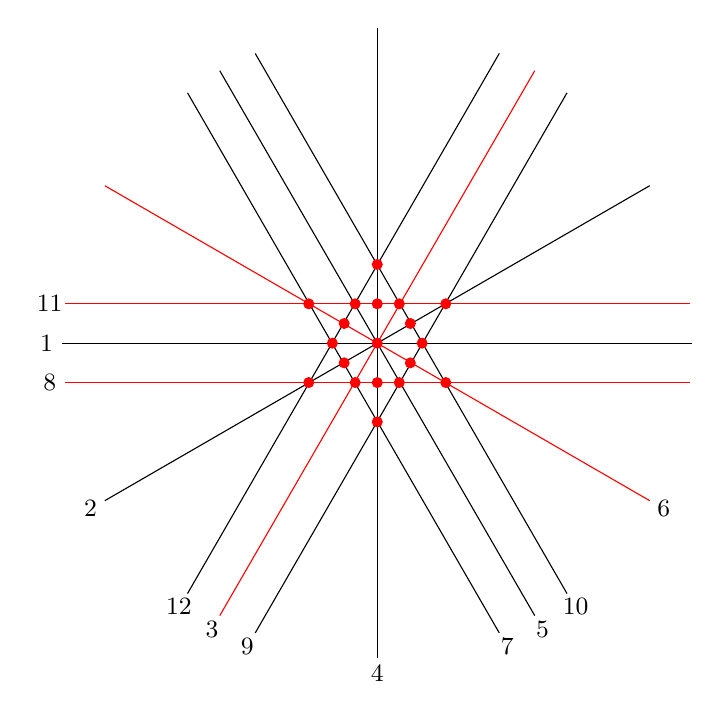
\begin{tikzpicture}[scale=1.0]
		\draw (4.,0.) -- (-4.,0.);  % H_1 
		\node at (-4.20,0.) {\small $1$}; 
		\draw (3.46,2.) -- (-3.46,-2.);  % H_2 
		\node at (-3.64,-2.10) {\small $2$}; 
		\draw[color=red] (2.,3.46) -- (-2.,-3.46);  % H_3 
		\node at (-2.10,-3.64) {\small $3$}; 
		\draw (0.,4.) -- (0.,-4.);  % H_4 
		\node at (0.,-4.20) {\small $4$}; 
		\draw (-2.,3.46) -- (2.,-3.46);  % H_5 
		\node at (2.10,-3.64) {\small $5$}; 
		\draw[color=red] (-3.46,2.) -- (3.46,-2.);  % H_6 
		\node at (3.64,-2.10) {\small $6$}; 
		\draw (-2.41,3.18) -- (1.55,-3.68);  % H_7 
		\node at (1.65,-3.85) {\small $7$}; 
		\draw[color=red] (3.97,-0.5) -- (-3.97,-0.5);  % H_8 
		\node at (-4.16,-0.5) {\small $8$}; 
		\draw (2.41,3.18) -- (-1.55,-3.68);  % H_9 
		\node at (-1.65,-3.85) {\small $9$}; 
		\draw (-1.55,3.68) -- (2.41,-3.18);  % H_10 
		\node at (2.52,-3.35) {\small $10$}; 
		\draw[color=red] (3.97,0.5) -- (-3.97,0.5);  % H_11 
		\node at (-4.16,0.5) {\small $11$}; 
		\draw (1.55,3.68) -- (-2.41,-3.18);  % H_12 
		\node at (-2.52,-3.35) {\small $12$}; 
		
		\fill[red] (0.0,0.0) circle[radius=2pt];  % P[ 1, 2, 3, 4, 5, 6 ] 
		\fill[red] (-0.57,0.0) circle[radius=2pt];  % P[ 1, 7, 12 ] 
		\fill[red] (-0.42,-0.25) circle[radius=2pt];  % P[ 2, 7 ] 
		\fill[red] (-0.28,-0.5) circle[radius=2pt];  % P[ 3, 7, 8 ] 
		\fill[red] (0.0,-1.) circle[radius=2pt];  % P[ 4, 7, 9 ] 
		\fill[red] (-0.87,0.5) circle[radius=2pt];  % P[ 6, 7, 11 ] 
		\fill[red] (-0.87,-0.5) circle[radius=2pt];  % P[ 2, 8, 12 ] 
		\fill[red] (0.0,-0.5) circle[radius=2pt];  % P[ 4, 8 ] 
		\fill[red] (0.28,-0.5) circle[radius=2pt];  % P[ 5, 8, 9 ] 
		\fill[red] (0.87,-0.5) circle[radius=2pt];  % P[ 6, 8, 10 ] 
		\fill[red] (0.57,0.0) circle[radius=2pt];  % P[ 1, 9, 10 ] 
		\fill[red] (0.87,0.5) circle[radius=2pt];  % P[ 2, 9, 11 ] 
		\fill[red] (0.42,-0.25) circle[radius=2pt];  % P[ 6, 9 ] 
		\fill[red] (0.42,0.25) circle[radius=2pt];  % P[ 2, 10 ] 
		\fill[red] (0.28,0.5) circle[radius=2pt];  % P[ 3, 10, 11 ] 
		\fill[red] (0.0,1.) circle[radius=2pt];  % P[ 4, 10, 12 ] 
		\fill[red] (0.0,0.5) circle[radius=2pt];  % P[ 4, 11 ] 
		\fill[red] (-0.28,0.5) circle[radius=2pt];  % P[ 5, 11, 12 ] 
		\fill[red] (-0.42,0.25) circle[radius=2pt];  % P[ 6, 12 ] 
		
	\end{tikzpicture}
	
	
	
	\end{center}
	\par
	Projective pictures produced by \texttt{LaTeXDrawProjPicture}.
	\end{figure}
	
	
	
\end{document}